Gating is a technique used to eliminate extremely unlikely observation-to-track pairings. A gate is calculated around the output of the Kalman filter (predicted position), and any observation outside of this gate is not further consider for that track. Furthermore if only one observation is found within the gate, then the observation is assigned directly to that track and no further processing is required (see \cref{mtt:assign}). 

\begin{figure}[h]
	\centering
	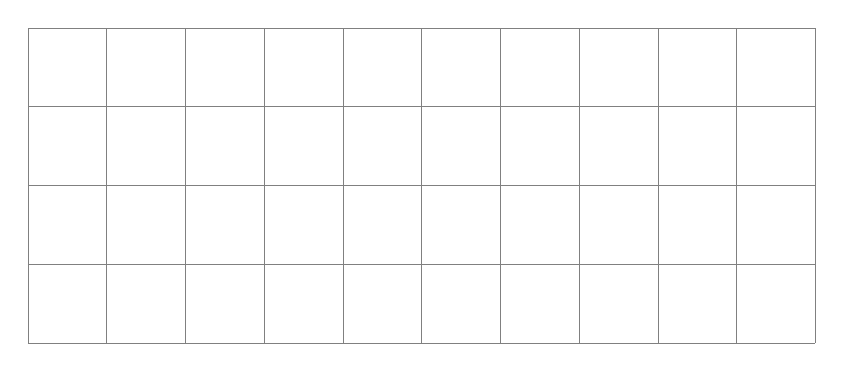
\begin{tikzpicture}
% Reference Grid
\draw[gray,very thin] (0,0) grid (10,4); 

\end{tikzpicture}
	\caption{Gating}
	\label{fig:gating}
\end{figure} 


One of the simplest gating techniques is using rectangular gates. A given observation is also said to satisfy the gates of a given track if the all the elements of the innovation vector satisfy 
\begin{equation}
	|\vec{v}(n)| \leq K_G \sigma_r
\end{equation}
where $\sigma_r$ is the residual standard deviation that can be expressed in terms of measurement $\sigma_o^2$ and prediction $\sigma_p^2$
\begin{equation}
	\sigma_r = \sqrt{\sigma_o^2 +\sigma_p^2}\\.
\end{equation}
Note that the values $\sigma_o$ and $\sigma_p$ can be found in the Kalman filter equations as 
\begin{align}
	\sigma_o &= R_{11} & \sigma_p &= P_{11}
\end{align}
The constant $K_G$ can be chosen freely. Usually, a Gaussian error model is assumed to that choosing $K_G = 3$ leads to the probability of a valid observation  satisfying the gating test to be about 99 percent. 